\documentclass{beamer}[10]
\usepackage{pgf}
\usepackage[danish]{babel}
\usepackage[utf8]{inputenc}
\usepackage{beamerthemesplit}
\usepackage{graphics,epsfig, subfigure}
\usepackage{url}
\usepackage{srcltx}
\usepackage{hyperref}
\usepackage{graphicx}

\graphicspath{ {images/} }

\definecolor{kugreen}{RGB}{0,53,24}
\definecolor{kugreenlys}{RGB}{132,158,139}
\definecolor{kugreenlyslys}{RGB}{173,190,177}
\definecolor{kugreenlyslyslys}{RGB}{214,223,216}
\setbeamercovered{transparent}
\mode<presentation>
\usetheme{PaloAlto}
\setbeamertemplate{footline}[frame number]

  \usecolortheme[named=kugreenlys]{structure}
  \useinnertheme{circles}
  \usefonttheme[onlymath]{serif}
  \setbeamercovered{transparent}
  \setbeamertemplate{blocks}[rounded][shadow=true]

\logo{
\includegraphics[width=1.5cm]{Uoseal.png}}
%\useoutertheme{infolines} 
\title{}
\subtitle{Using Statistical Distributions to Generate Random Test Data}
\author{Jamie L. Zimmerman}
\institute{Robert D. Clark Honors College \\ Department of Computer and Information Science \\ University of Oregon}
\date{25 May 2018}

\AtBeginSection[]
{
  \begin{frame}
    \frametitle{Overview}
    \tableofcontents[currentsection]
  \end{frame}
}


\begin{document}
\frame{\titlepage \vspace{-0.5cm}
}


% Introduction
\section{Introduction}

\frame{
\frametitle{What is Software Testing?}
\begin{figure}
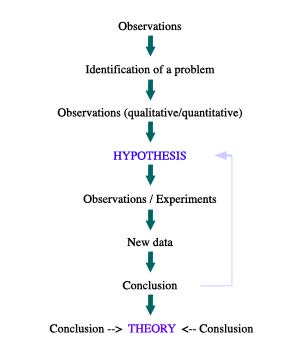
\includegraphics[scale=0.55]{scientific-method}
\end{figure}
}

\frame{
\frametitle{Why is it so hard?}
\begin{figure}
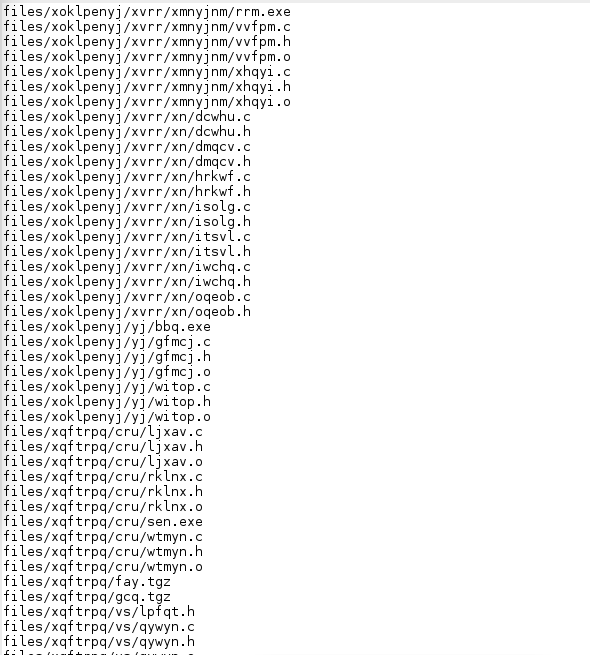
\includegraphics[scale=0.3]{file-listing.png}
\end{figure}
}

\frame{
\frametitle{}
\begin{figure}
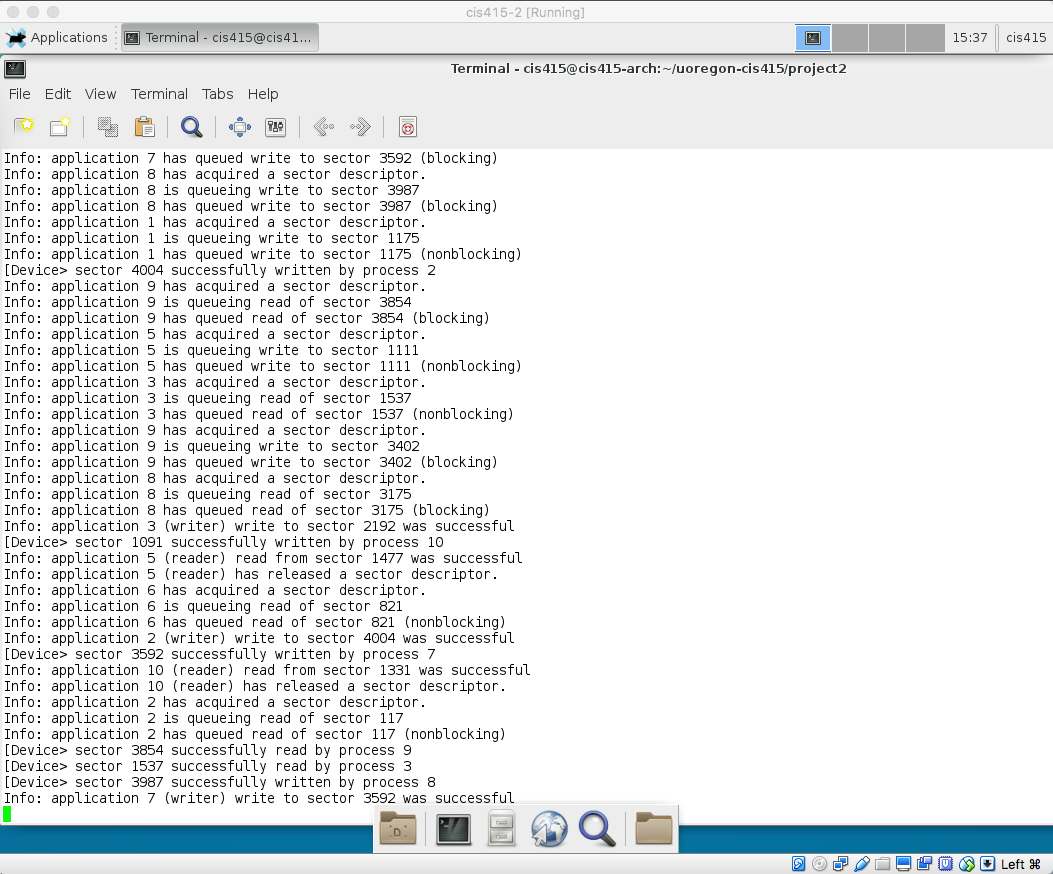
\includegraphics[scale=0.25]{complicated_output.png}
\end{figure}
}

\frame{
\frametitle{}
\begin{figure}
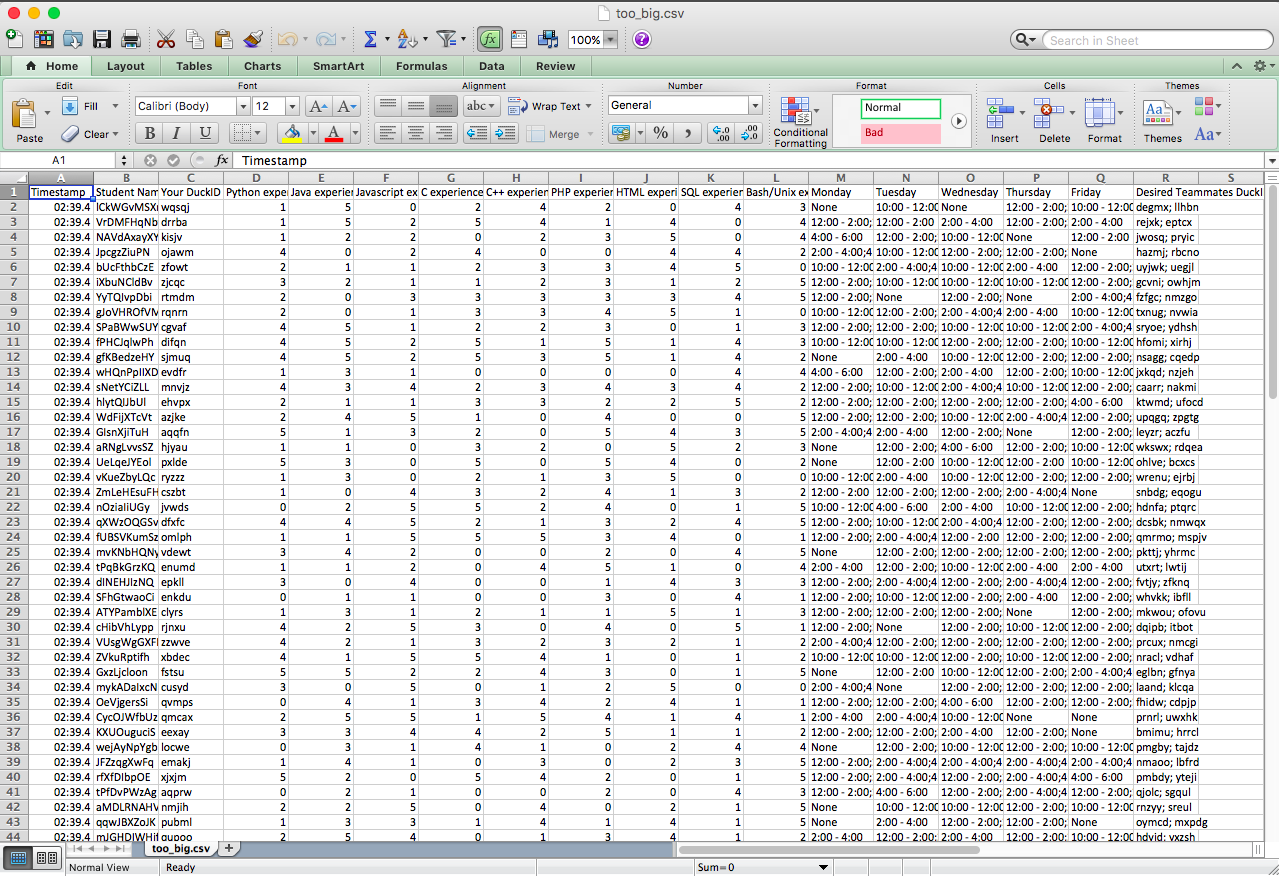
\includegraphics[scale=0.22]{input.png}
\end{figure}
}

\frame{
\frametitle{}
\begin{figure}
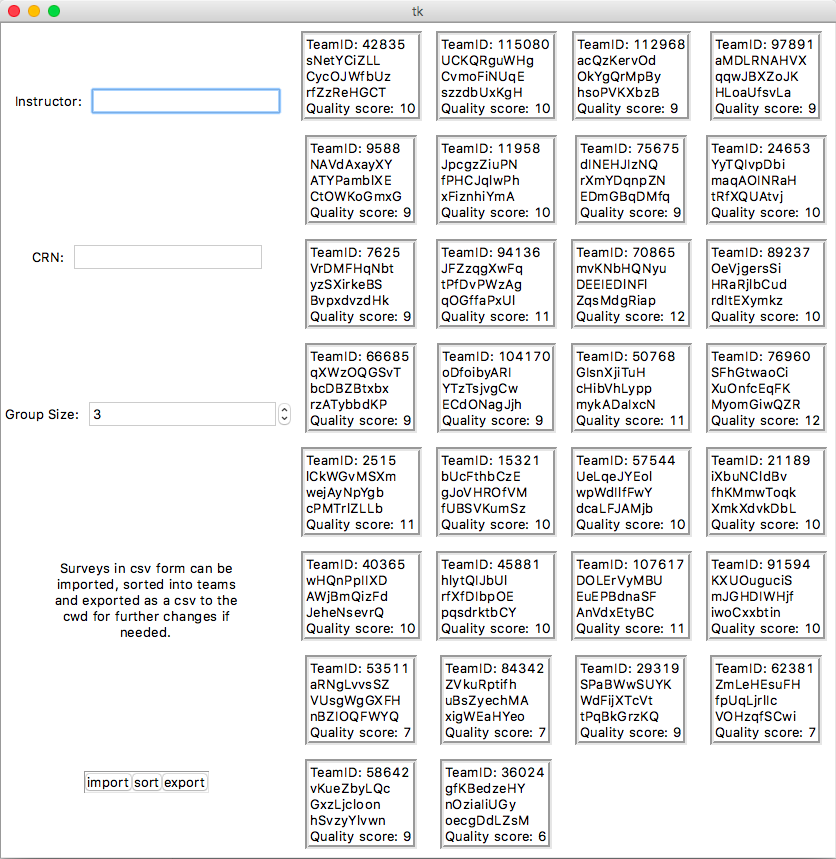
\includegraphics[scale=0.25]{output.png}
\end{figure}
}

\frame{
\frametitle{}
\begin{figure}
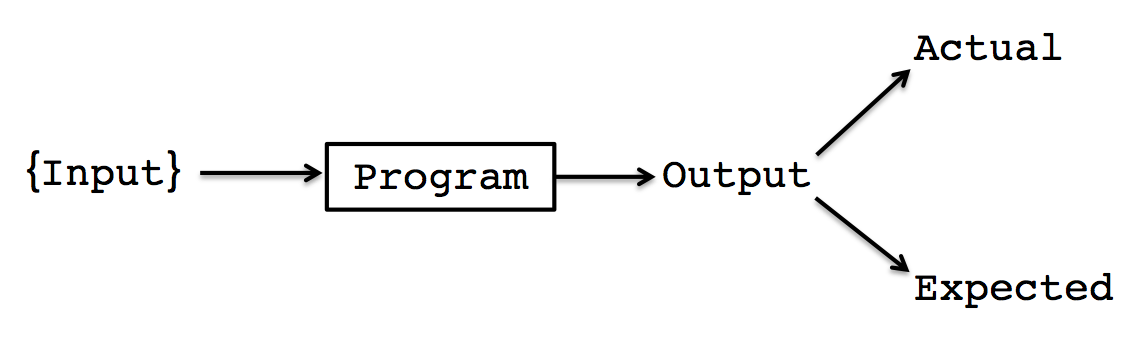
\includegraphics[scale=0.5]{diagram.png}
\end{figure}
}

\frame{
\frametitle{Well if it's so hard why bother?}
\begin{figure}
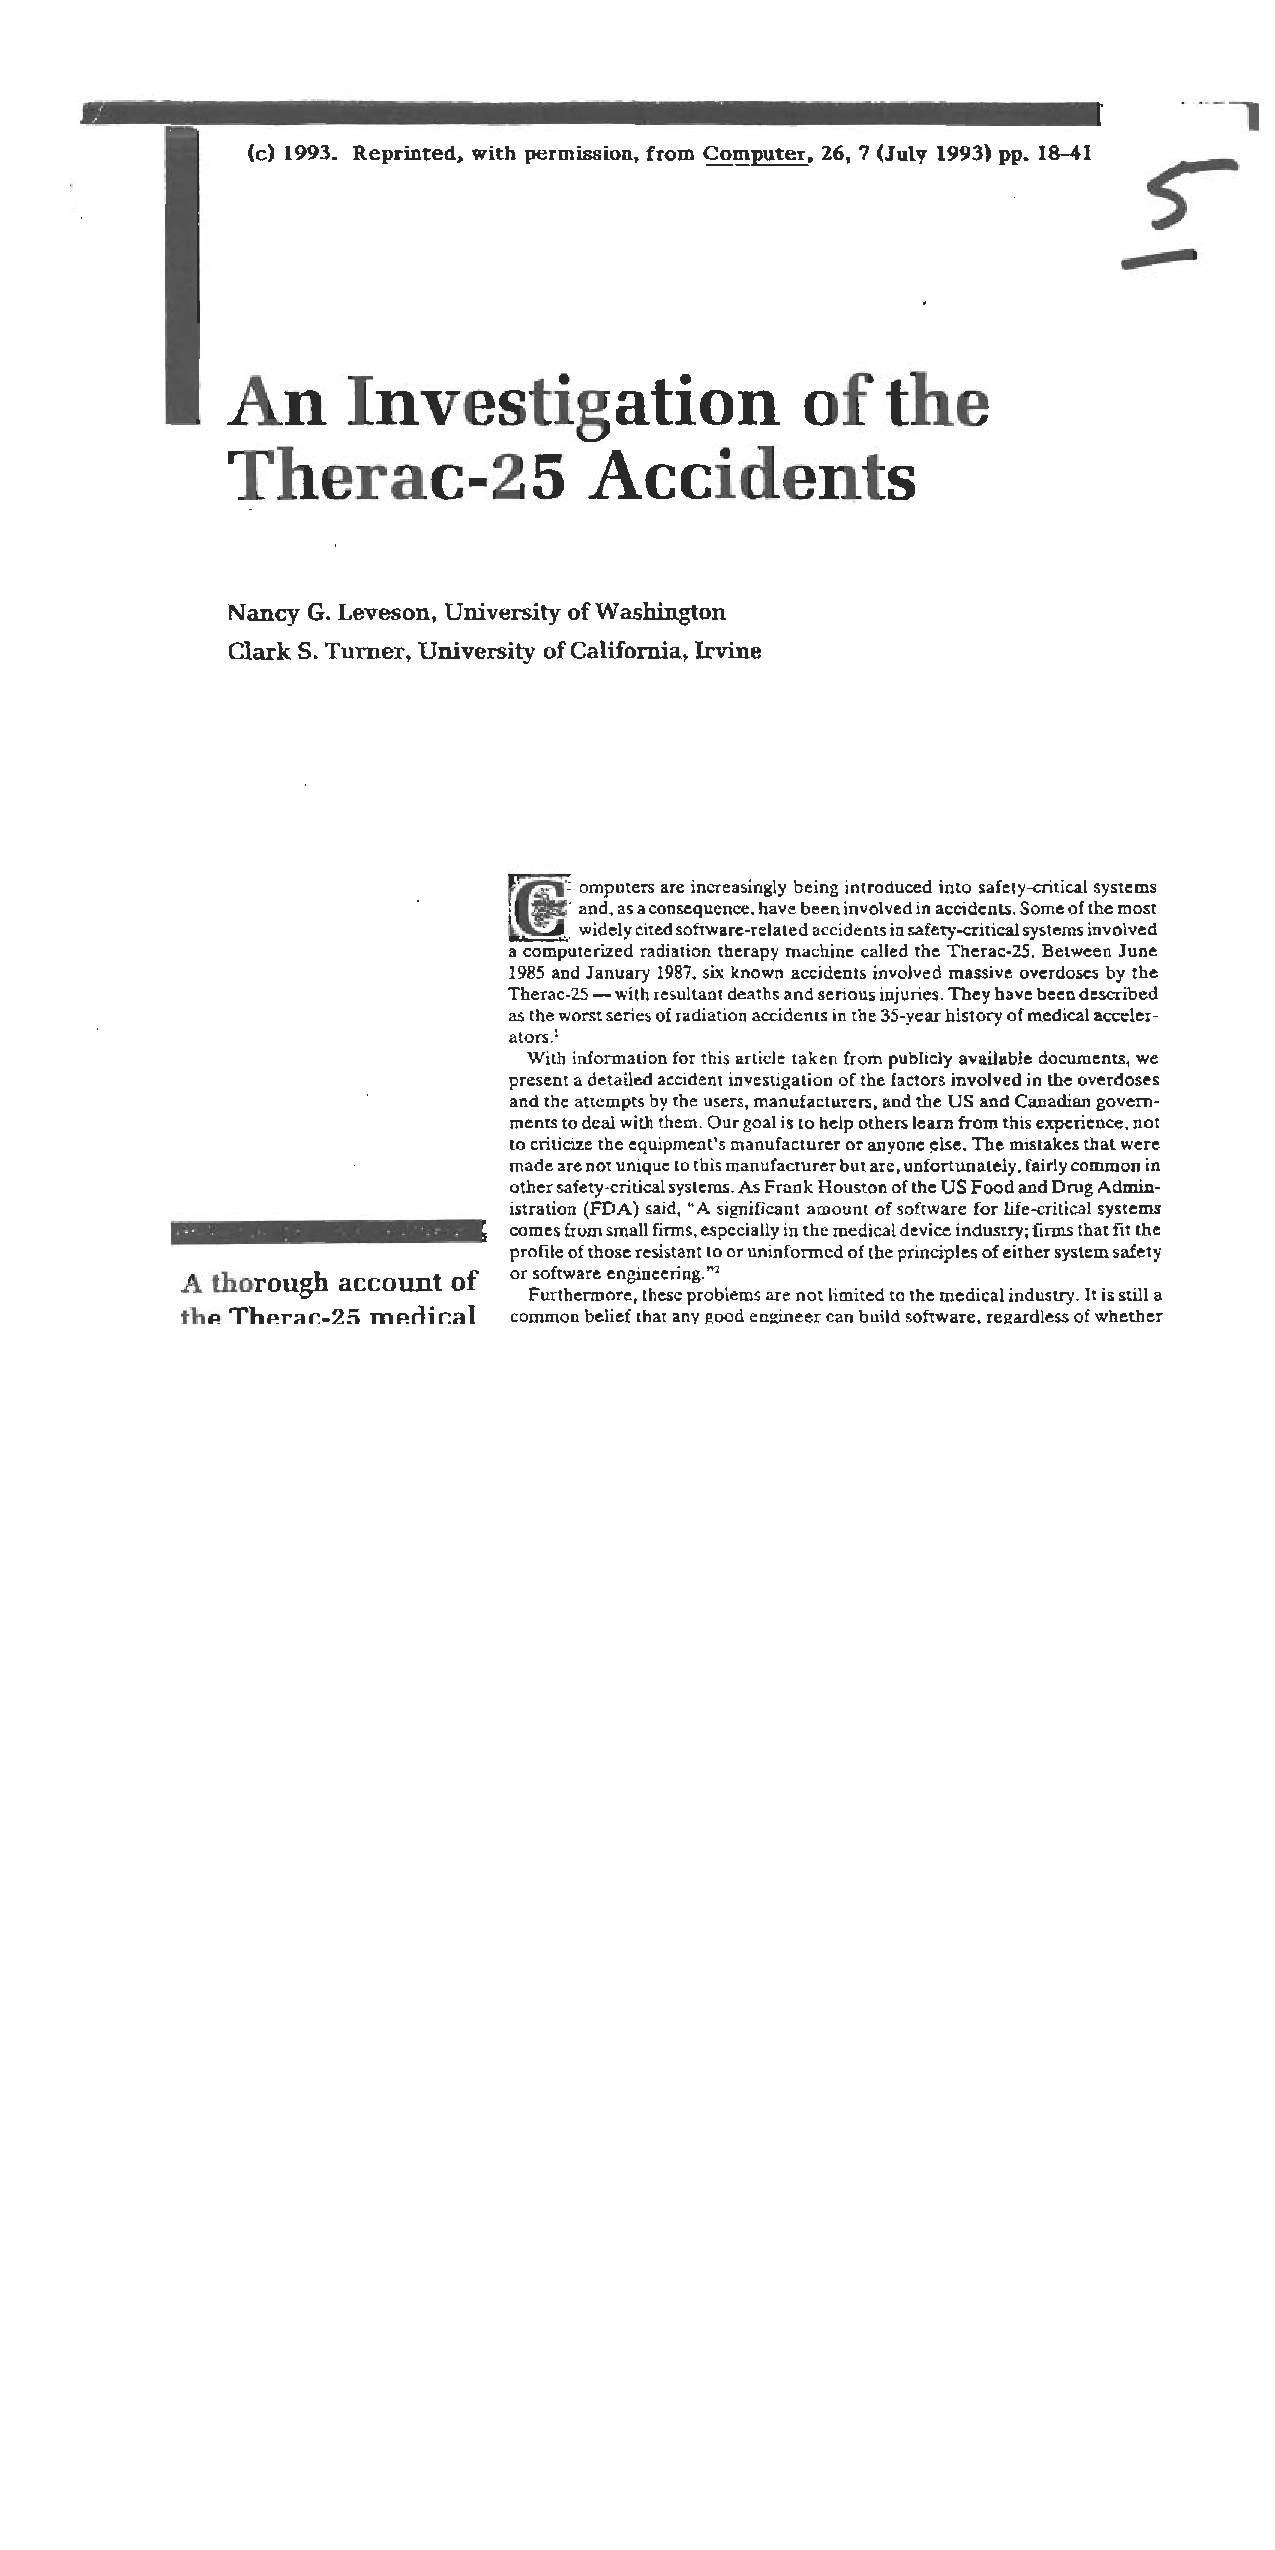
\includegraphics[scale=0.45]{therac-25.pdf}
\end{figure}
}

% Hypothesis
\section{Proposed Argument}

\frame{
\frametitle{GenSequence}
\begin{figure}
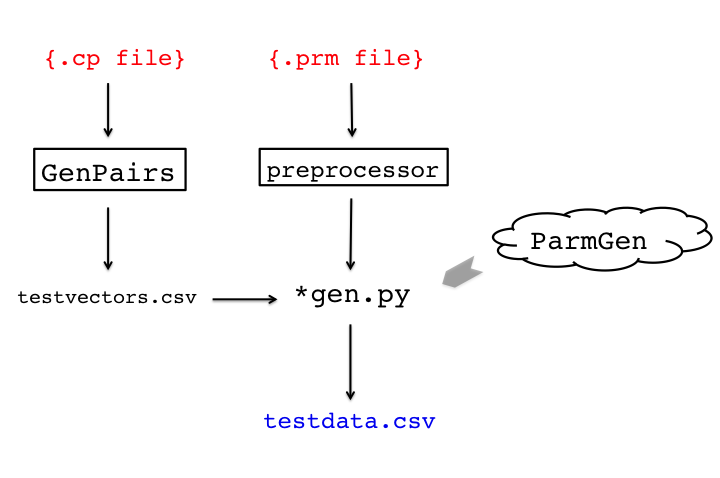
\includegraphics[scale=0.4]{workflow.png}
\end{figure}
}

\frame{
\frametitle{Goals}
\begin{itemize}
\item Ease of use - as much end-to-end automation as possible
\item Insight into what the input looks like
\end{itemize}
}

% Design Decisions
\section{Architecture}

\frame{
\frametitle{Pairwise Testing}
\begin{figure}
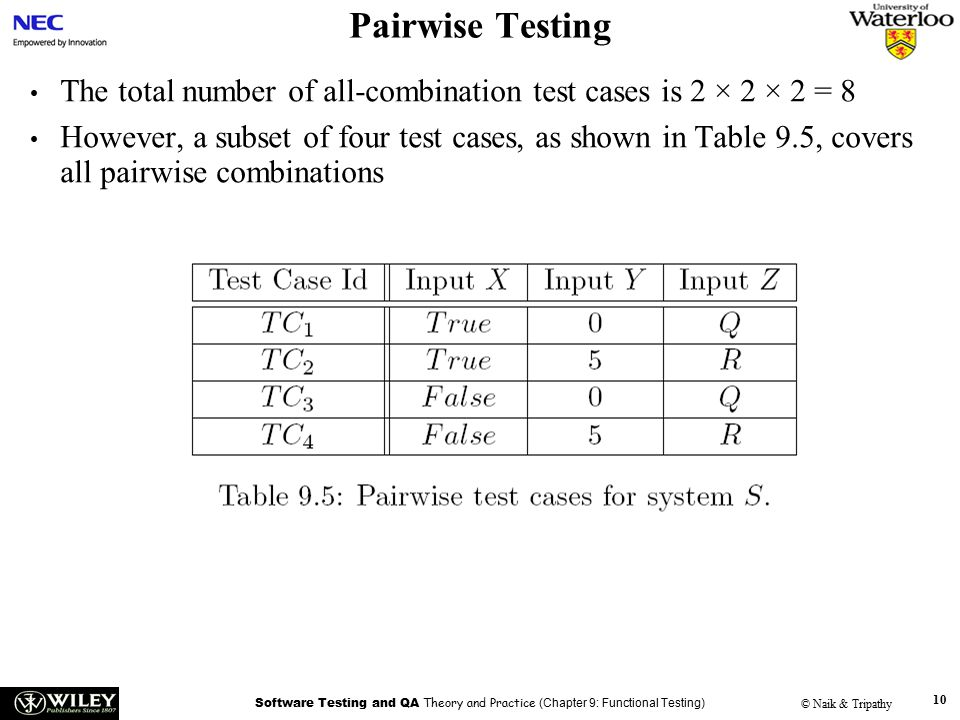
\includegraphics[scale=0.4]{pairwise.jpg}
\end{figure}
}

\frame{
\frametitle{ParmGen}
Constrained Randomness
}

\frame{
\frametitle{100 points}
\begin{figure}
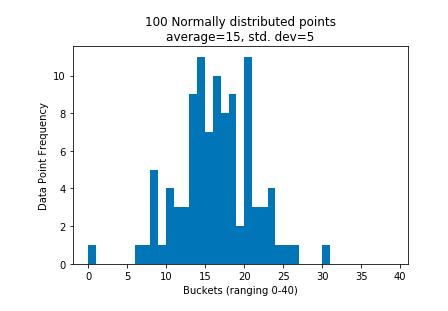
\includegraphics[scale=0.6]{law1.png}
\end{figure}
}

\frame{
\frametitle{Law of Large Numbers}
\begin{itemize}
\item Bernoulli's Principle
\item Selection Scheme
\end{itemize}
}

\frame{
\frametitle{10,000 points}
\begin{figure}
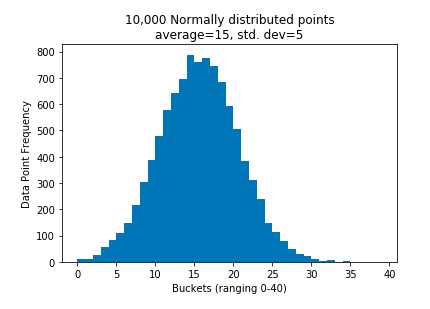
\includegraphics[scale=0.6]{law2.png}
\end{figure}
}

\frame{
\frametitle{300 points}
\begin{figure}
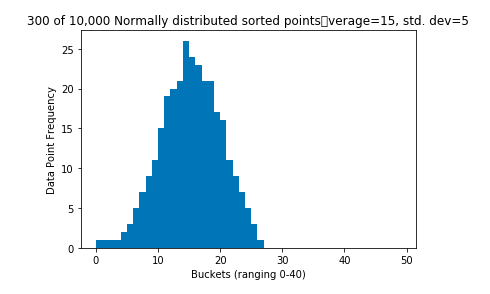
\includegraphics[scale=0.6]{law3.png}
\end{figure}
}

\frame{
\frametitle{Cardioids}
$$r = \alpha \pm \alpha cos \theta$$
\begin{figure}
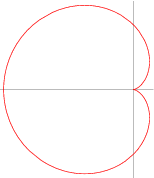
\includegraphics[scale=0.9]{cardioid.png}
\end{figure}
}


\section{Results}

\frame{
\frametitle{Orbits Simulation}
13-70-mass$|$right\_slanted-position$|$right\_slanted-velocity$|$uniform-diameter$|$left\_slanted.csv
\begin{itemize}
\item Case 13
\item 70 bodies
\item Mass - right-slant
\item Position - right-slant
\item Velocity - uniform
\item Diameter - left-slant
\end{itemize}
}

\frame{
\frametitle{Starting Orbits}
\begin{figure}
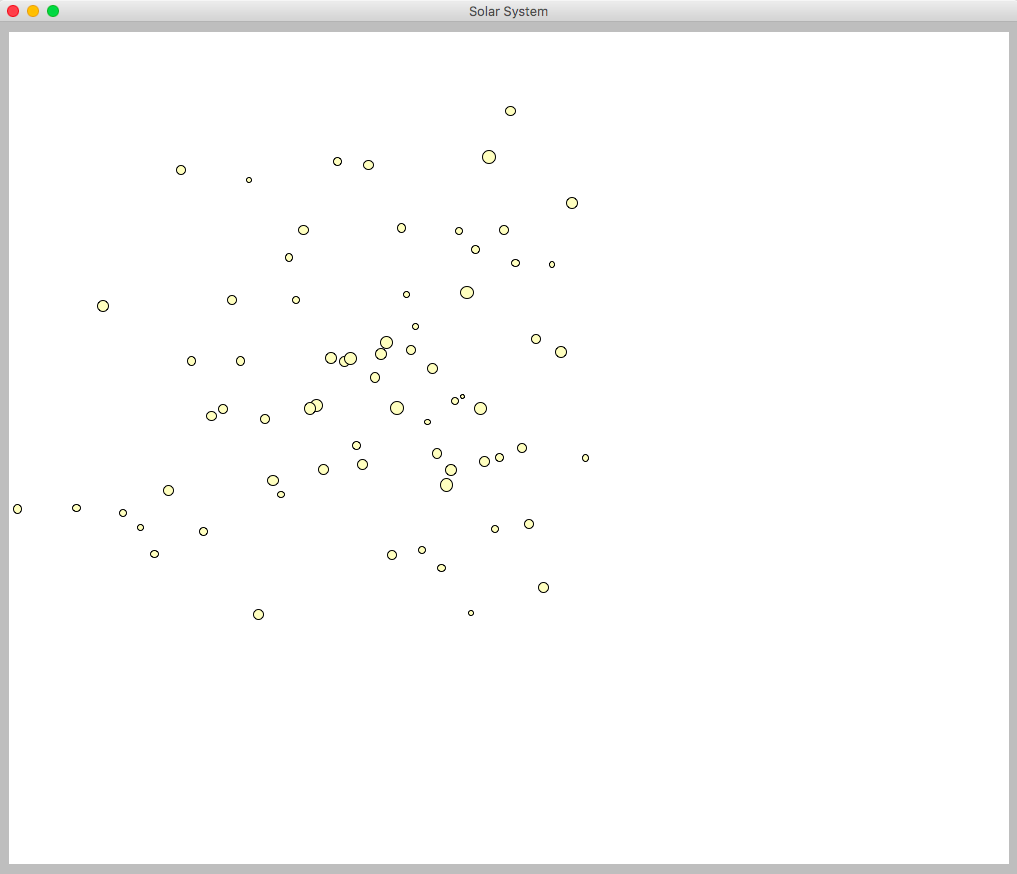
\includegraphics[scale=0.21]{start-ex.png}
\end{figure}
}

\frame{
\frametitle{Starting Observations}
\begin{itemize}
\item Sizes are mostly small-medium (from left-slant distribution)
\item Locations are clustered (from right-slant distribution)
\end{itemize}
}

\frame{
\frametitle{Ending Orbits}
665 time steps
\begin{figure}
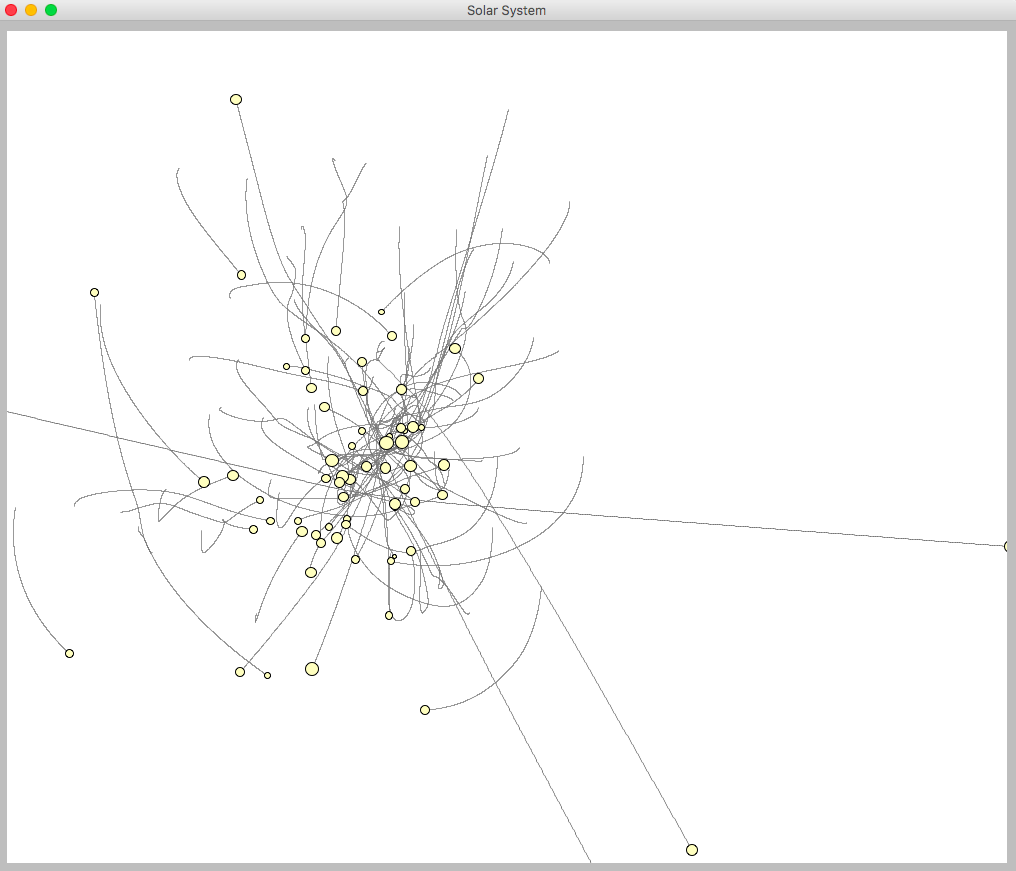
\includegraphics[scale=0.21]{final-ex.png}
\end{figure}
}

\frame{
\frametitle{Ending Observations}
\begin{itemize}
\item Behavior of gravity 
\item Path lengths are all different (from uniform velocity)
\end{itemize}
}

\frame{
\frametitle{Earthquake Analysis}
6-70-magnitudes$|$cardioid-latitudes$|$left\_slanted-longitudes$|$right\_slanted-depths$|$cardioid.csv
\begin{itemize}
\item Case 6
\item 70 quake events
\item Magnitude \& Depth - Cardioid relationship
\item {Trend: High Magnitude $\to$ High Depth
\item Low Magnitude $\to$ Low Depth}
\item Latitudes - left-slant
\item Longitudes - right-slant
\end{itemize}
}

\frame{
\frametitle{Magnitudes \& Depths}
\begin{figure}
\subfigure[Magnitudes]{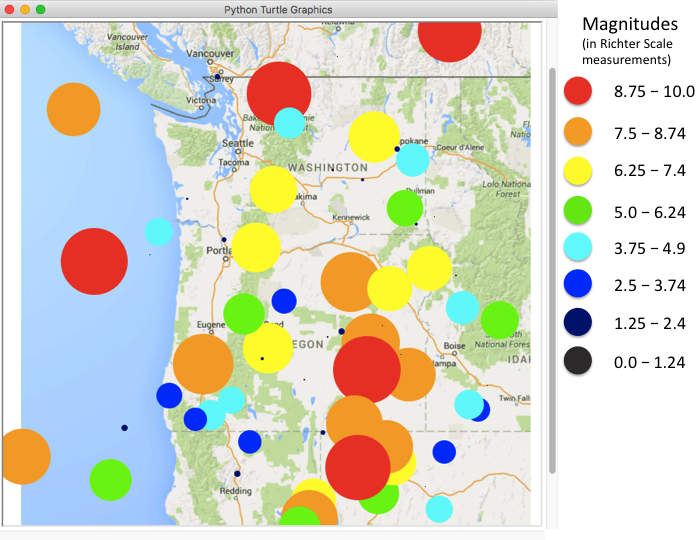
\includegraphics[scale=0.19]{mags.png}}
\hfill
\subfigure[Depths]{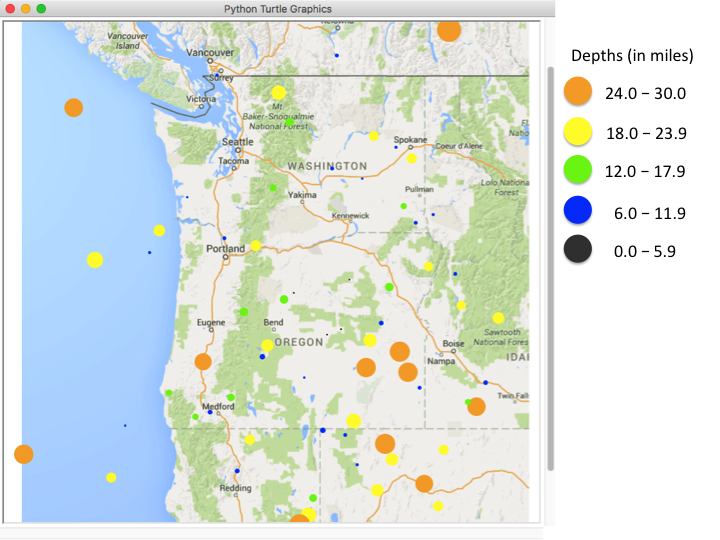
\includegraphics[scale=0.19]{depths.png}}
\end{figure}

}

\frame{
\frametitle{Observations}
\begin{itemize}
\item Mostly predicted events?
\item Any outliers?
\end{itemize}
}

\frame{
\frametitle{Predict}
\begin{itemize}
\item North - Up
\item West - Left
\item East - Right
\item South - Down
\item right-slanted is high numbers
\item left-slanted is low numbers
\item right-leaning longitudes
\item left-leaning latitudes
\item Quakes drift towards lower-right corner
\end{itemize}
}

\frame{
\frametitle{Latitudes \& Longitudes}
\begin{figure}
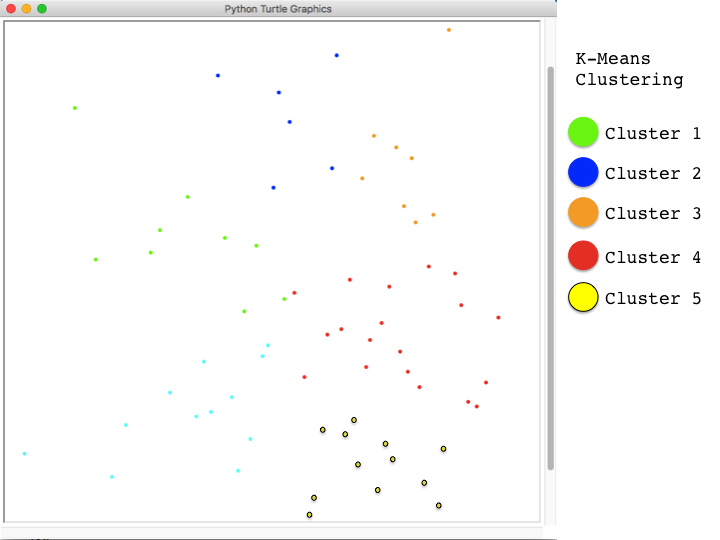
\includegraphics[scale=0.3]{clusters-nobg.png}
\end{figure}
}

\section{Concluding Thoughts}
\frame{
\frametitle{GenSequence in all its Power}
\begin{itemize}
\item It is what it says it is
\item Nearly end-to-end automation
\item Knowing about input informs the expected output?
\end{itemize}
}


\frame{
\frametitle{Future Work}
\begin{itemize}
\item Test GenSequence against an open-source project
\item Machine Learning Models
\item Database-Driven Applications
\item Combine user-written spec files
\end{itemize}
}

\end{document}
